\chapter{Overall Description}
\lhead{\thechapter \space Overall Description}
\label{ch:overall_description}

\section{Product Perspective}
%TO DO: Explain whether or not the product is part of a larger system. In case it is, explain how this product will contribute to the larger system's requirements and identify interfaces between this product and the rest of the system. Using diagrams to elaborate is helpful
The product will be developed as a first step of a larger project, which ultimately has the goal to semi-automate the cycle count processes of the inventory control \& management department of the customer's warehouses. The concept was initially developed in order to combat the increasing scarceness of warehouse cycle count employees. An overview of the larger project can be found in figure \ref{fig:roadmap}.

\paragraph{System Interfaces}
As the product for which this document is written will be the first component of the Seacon Drone project, the interfaces of the Seacon Drone project which the product will communicate with have yet to be defined.

\paragraph{Hardware Interfaces}
The product will support Dji Tello drones \citep{tello}. It will developed to be used with a Wi-Fi enabled laptop. The product will provide a set of drone control command keys, which will only work as intended on an QWERTY or AZERTY keyboard layout.

\paragraph{Software Interfaces}
The product will be developed in Ubuntu 18.04. This will thus be the only operating system and version which will have guaranteed support. Furthermore, the device running the product is required to have a python interpreter version 3.6.x with pip, as this will be the language and package management system for development, respectively. The python-pip packages the software will make use of are:
\begin{itemize}
	\item opencv-python (version 4.1.1.26) \citep{opencv}
	\item av (version 6.2.0) \citep{av}
	\item tellopy (version 0.6.0) \citep{tellopy}
	\item simple\_pid (version 0.2.4) \citep{pid}
	\item pynput (version 1.4.5) \citep{pynput}
\end{itemize}

\begin{figure}[ht]
	\centering
	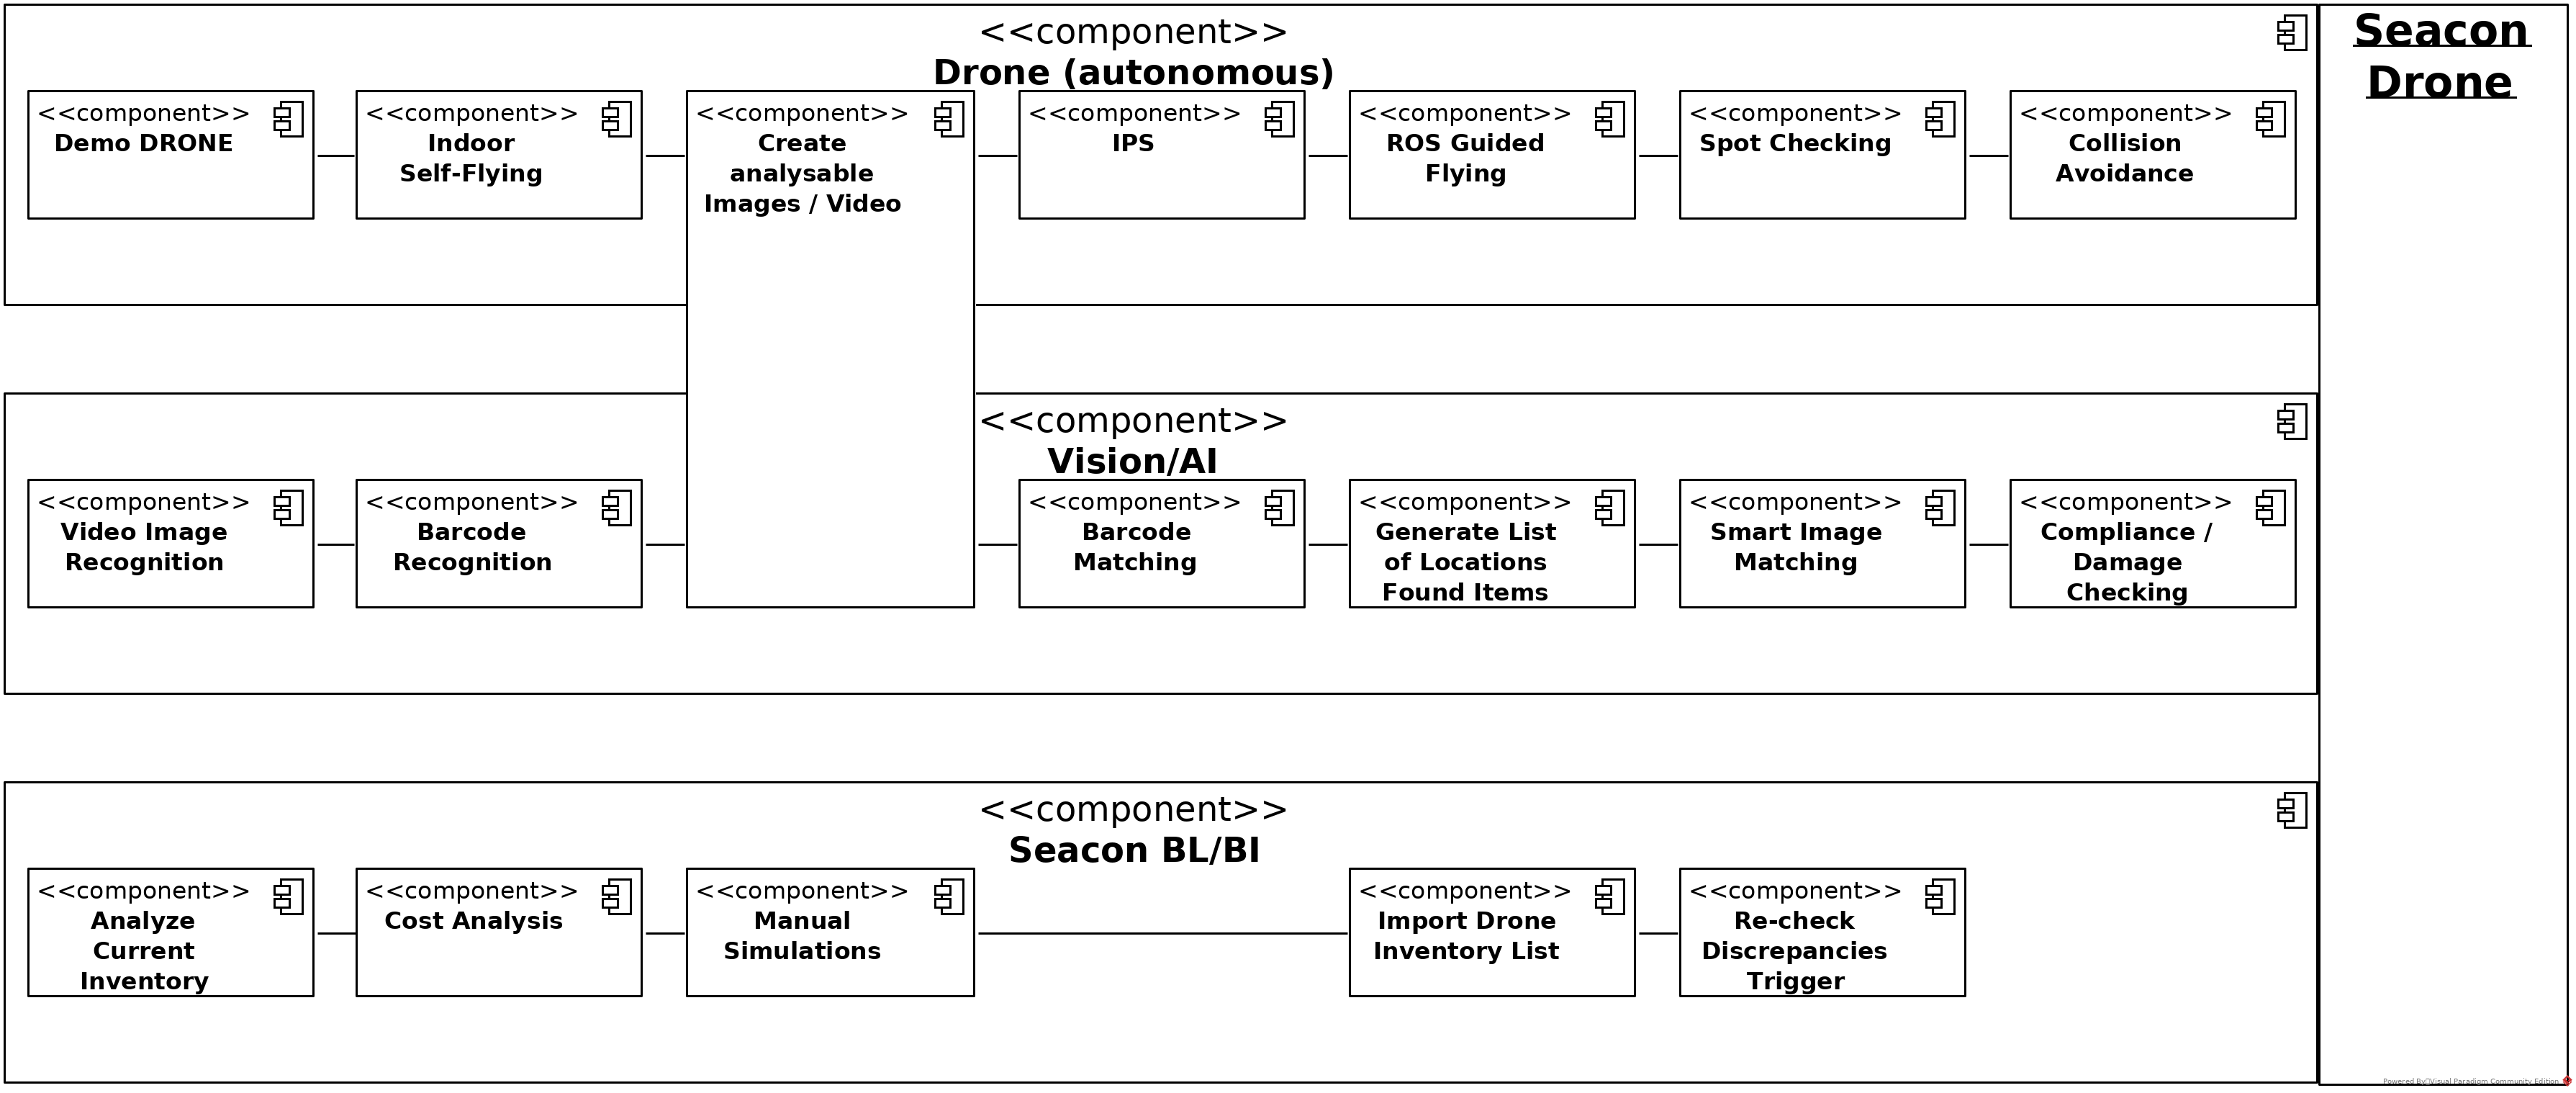
\includegraphics[width=\linewidth]{img/seacon_roadmap.png}
	\label{fig:roadmap}
	\caption{Roadmap of the Seacon Drone Project}
\end{figure}
\pagebreak
\section{Product Functions}
The product can be divided into 3 parts: x-axis, y-axis, z-axis of the drone. Each axis can then be subdivided further into a video processing part, drone movement part, and a collision avoidance part. Figure \ref{fig:drone_concept} visualizes those 3 axes.
\begin{figure}[h]
	\centering
	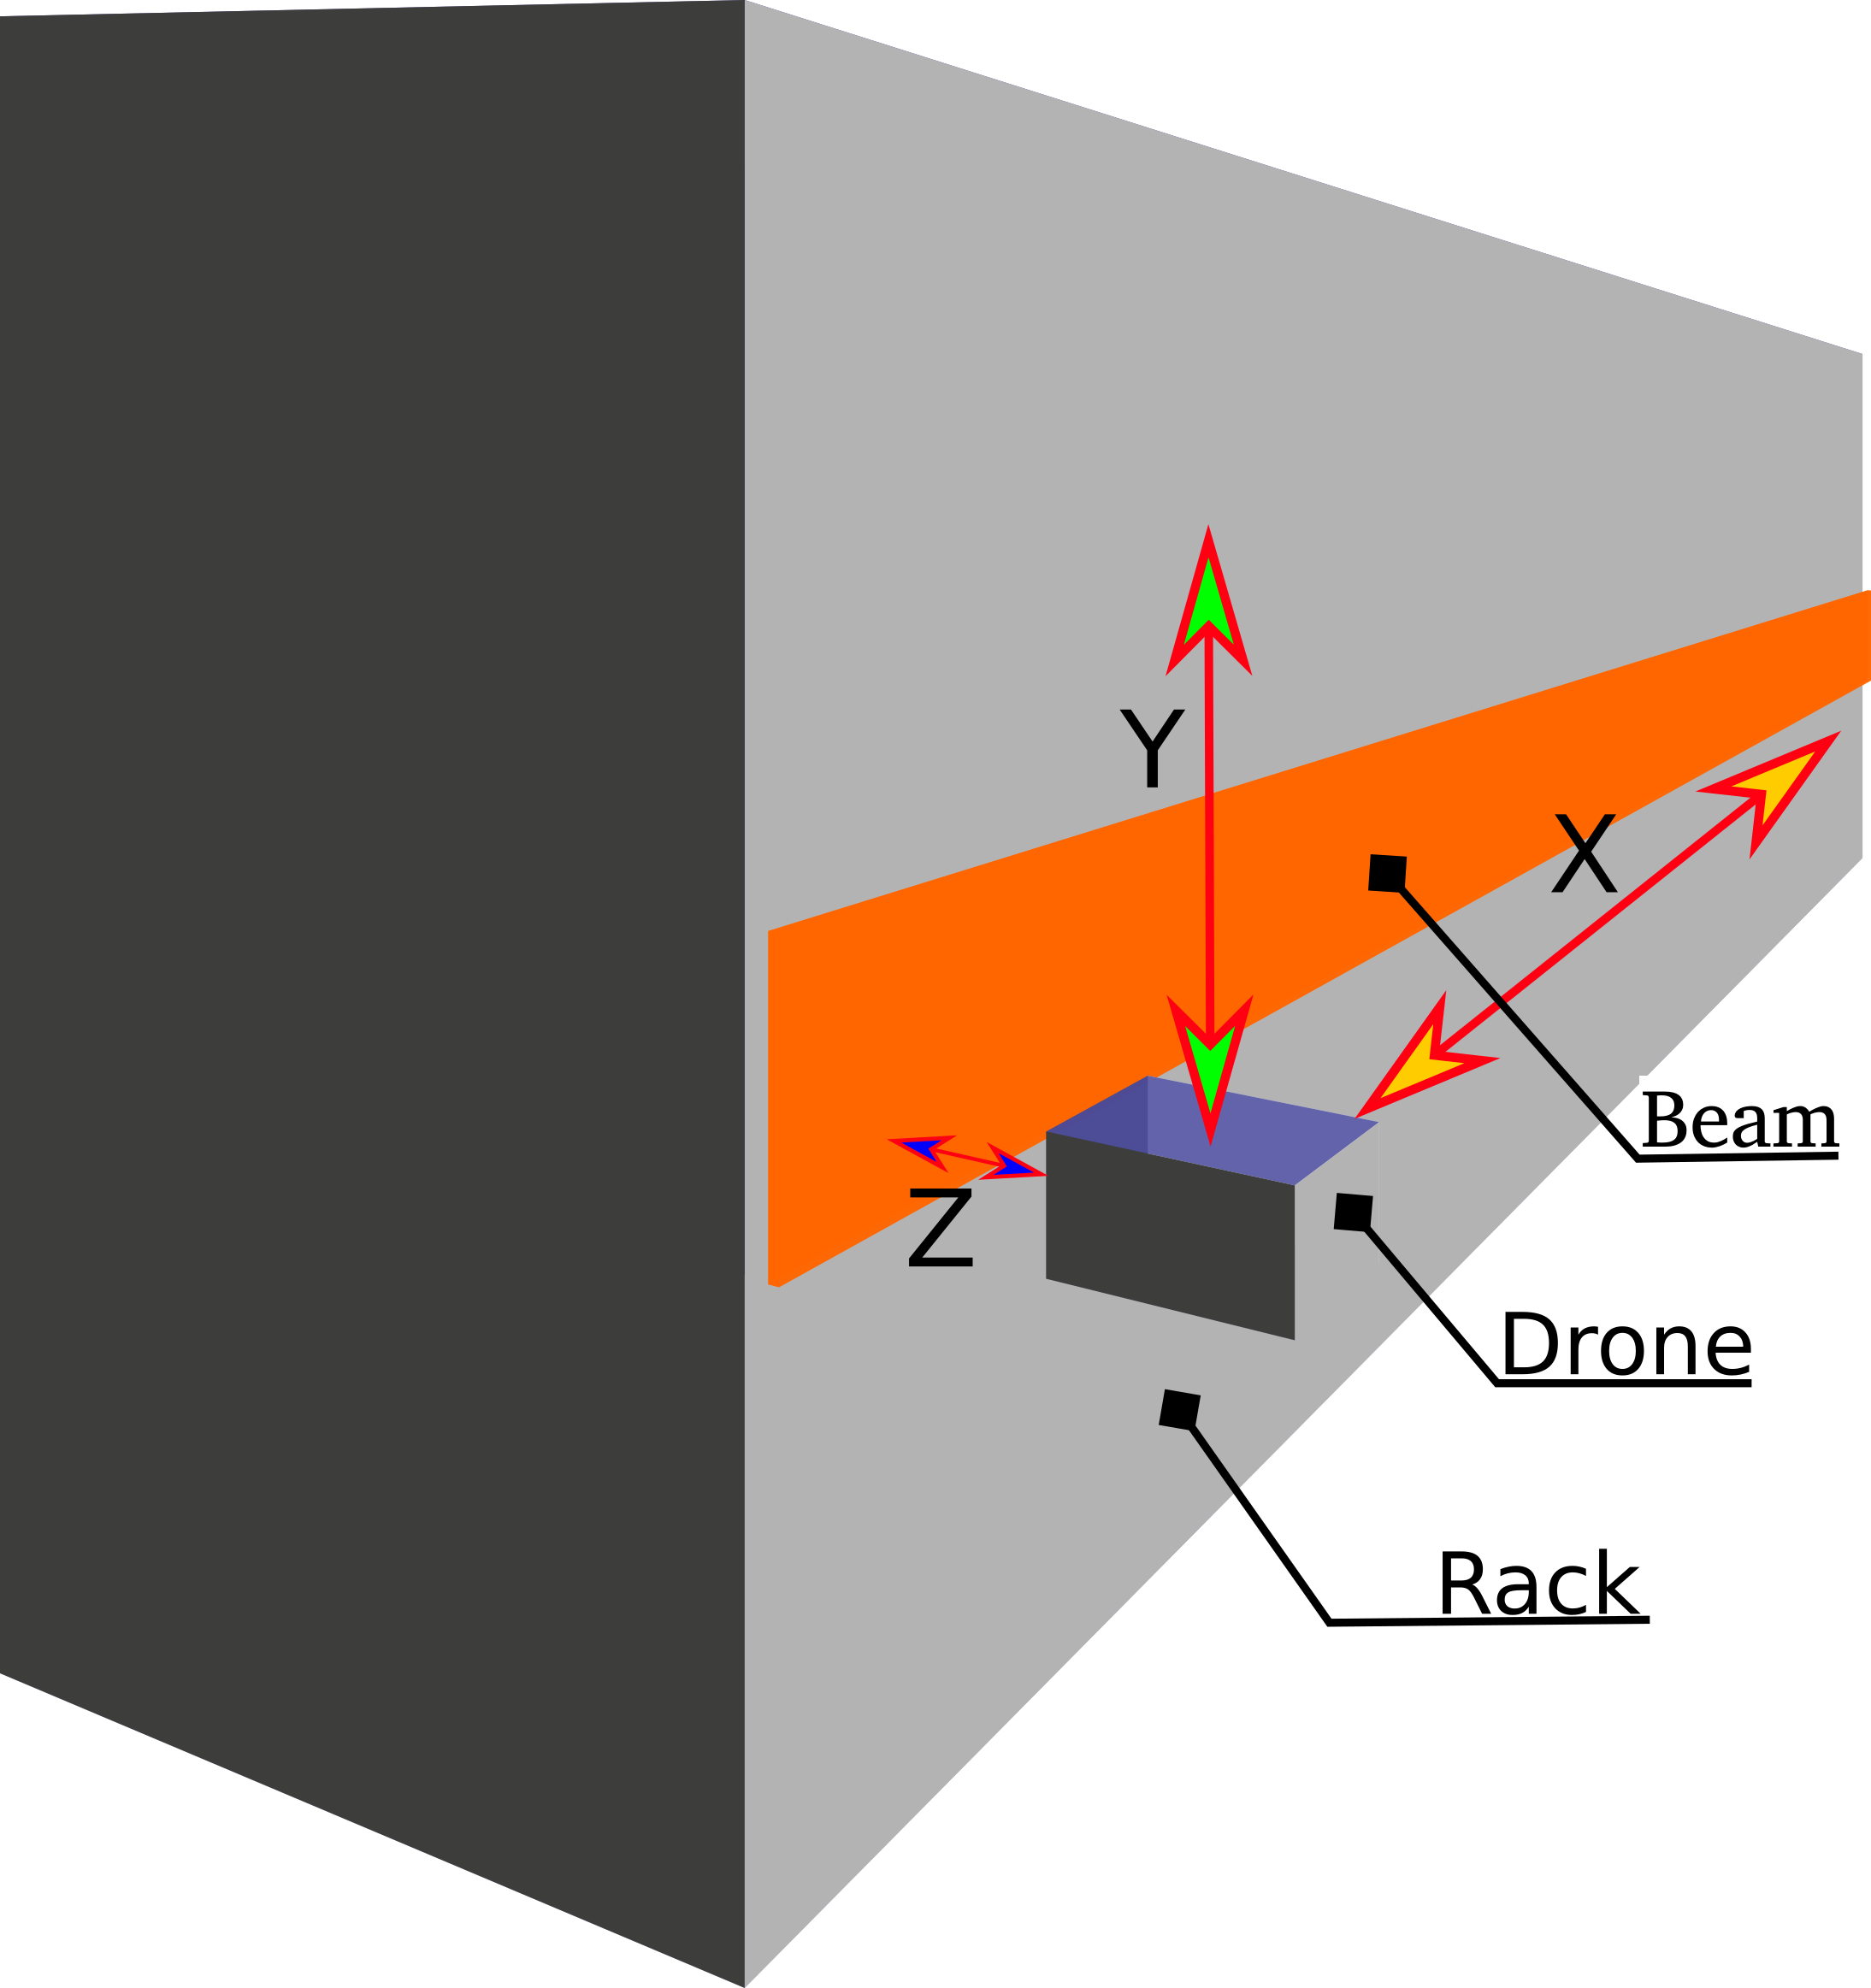
\includegraphics[width=\linewidth/2]{img/drone_concept_diagram.png}
	\label{fig:drone_concept}
	\caption{Simple drawing visualizing the intended product.}
\end{figure}
\pagebreak
\begin{itemize}
	\item X-axis:
	\begin{itemize}
		\itemsep0em
		\item Move the drone sideways
		\item Stop the drone at the end of a bar
		\item Detect objects in the drone's trajectory
		\item Avoid collisions with objects in the drone's trajectory
	\end{itemize}
	\item Y-axis:
	\begin{itemize}
		\itemsep0em
		\item Keep the bar in the center of the drone's camera
		\item Change the drone's altitude to switch layers
		\item Keep track of the current layer and the highest layer
	\end{itemize}
	\item Z-axis:
	\begin{itemize}
		\itemsep0em
		\item Estimate the pixel size of the bar
		\item Keep the drone to maintain distance from the bar
	\end{itemize}
\end{itemize}
When referring to "objects", one of the following things is meant:
\begin{itemize}
	\itemsep0em
	\item Pallets
	\item Racks
	\item Forklifts
	\item People
	\item Drones
\end{itemize}

\section{User Classes and Characteristics}
As the product of this iteration will not yet include inventory control functionality, the typical users do currently not include a warehouse employee class. Thus the sole user class of this product will be developers who aim to improve and/or extend the current product. Developers are required to have an extensive knowledge of Python and Opencv.


